\part{What is sound? What is a wave?}
\frame{\partpage}

\begin{frame}
	\begin{center}
		\textbf{Quick Definition:} A wave of compression and refraction in an elastic medium, such as air, which can be detected by an animal’s sense of hearing 
	\end{center}
\end{frame}

\begin{frame}{What is Sound?}
	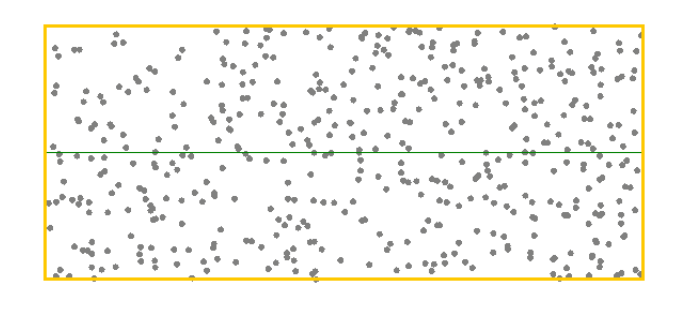
\includegraphics[width=\linewidth,height=0.8\textheight,keepaspectratio]{sound_molecules}
\end{frame}

\begin{frame}{What is a Wave?}
	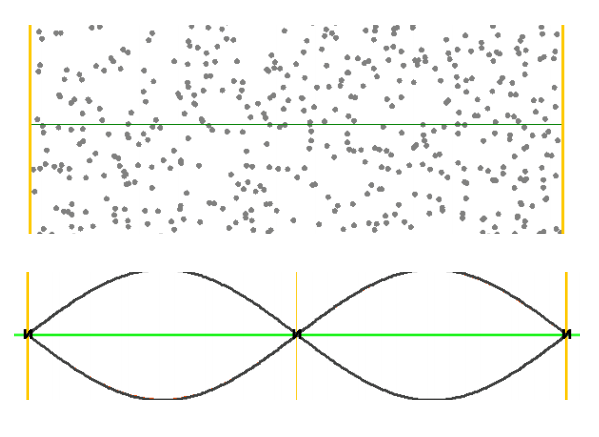
\includegraphics[width=\linewidth,height=0.8\textheight,keepaspectratio]{sound_wave}
\end{frame}

\begin{frame}{What is a Wave?}
	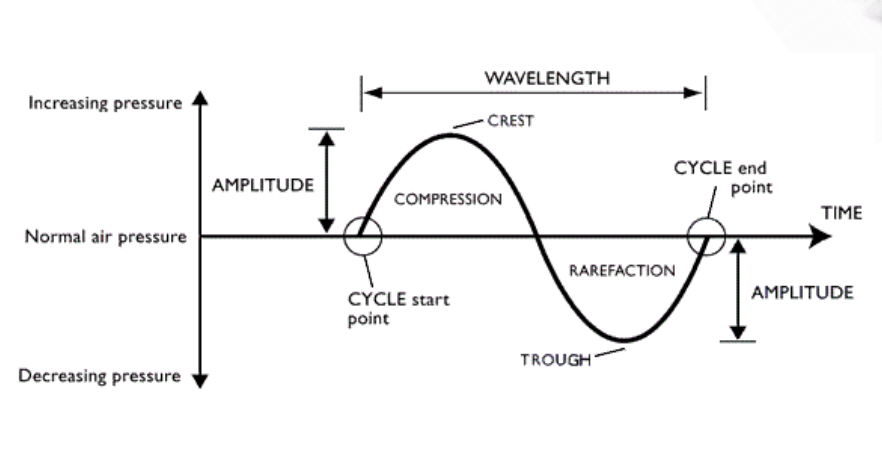
\includegraphics[width=\linewidth,height=0.8\textheight,keepaspectratio]{wave_desc}
\end{frame}

\begin{frame}{What is Sound?}
	\begin{itemize}
		\item Many animals are able to sense sound in two key ways:
		\textbf{volume} and \textbf{pitch}.
		\item\textbf{Volume:} The intensity of the change in pressure, as signified by the
		amplitude of a wave
		\item\textbf{Pitch:} The frequency of the change, as signified by the length of
		the wave and its velocity (i.e., “the speed of sound”)
	\end{itemize}
\end{frame}